\documentclass[12pt, a4paper, onecolumn, oneside, final]{report}

\usepackage{tocbibind}
\usepackage{natbib}

\usepackage{hyperref}
  \hypersetup{
  	colorlinks=false,
  	pdfborder=0 0 0,
  	linkcolor=blue,
  	citecolor=black,
  	bookmarksopen=false,
  	bookmarksnumbered=true,
  	pdfstartview=FitH,
  	pdfview=FitH
	}
	
\usepackage{url}
  \urlstyle{same}

\usepackage{fancyhdr}

\usepackage{amsmath}
\usepackage{amsfonts}
\usepackage{bm}

\usepackage{listings}
\usepackage{xcolor}
\usepackage{pdfpages}
\usepackage[bahasa]{babel}
\usepackage[fixlanguage]{babelbib}

\definecolor{codegreen}{rgb}{0,0.6,0}
\definecolor{codegray}{rgb}{0.5,0.5,0.5}
\definecolor{codepurple}{rgb}{0.58,0,0.82}
\definecolor{backcolour}{rgb}{0.95,0.95,0.92}

\lstdefinestyle{mystyle}{
    backgroundcolor=\color{backcolour},   
    commentstyle=\color{codegreen},
    keywordstyle=\color{magenta},
    numberstyle=\tiny\color{codegray},
    stringstyle=\color{codepurple},
    basicstyle=\ttfamily\footnotesize,
    breakatwhitespace=false,         
    breaklines=true,                 
    captionpos=b,           
    keepspaces=true,                 
    showspaces=false,                
    showstringspaces=false,
    showtabs=false,                  
    tabsize=2,
    numbers=none
}

\lstset{style=mystyle}

\title{Tugas Kelompok 1\\Aljabar Numerik Kelas A\\Tahun Ajaran 2020/2021}
\author{Eko Julianto Salim, Hocky Yudhiono, Jonathan Nicholas}

\begin{document}

\maketitle

\section*{Pendahuluan}

Berbagai permasalahan fisika yang ada di sekeliling kita tidak lepas dari perhitungan kontinu dan bilangan-bilangan nyata. Dalam menyusun persamaan dan menyelesaikan permasalahan tersebut, tidak selalu ditemukan metode analisis dalam menghitung secara pasti.

Matematikawan dan ilmuwan komputer sejak dulu sudah meneliti berbagai cara untuk melakukan komputasi dan mengembangkan algoritme-algoritme yang dapat menghitung dan menyelesaikan permasalahan matematika secara cepat. Meskipun solusi yang ditemukan secara esensial merupakan aproksimasi dari solusi sesungguhnya, berbagai solusi dengan galat yang lebih kecil masih terus dicari dengan berbagai teknik komputasi.

Di era modern ini, ilmu komputer dan informatika berkembang cepat. Manusia dapat menghitung berbagai masalah matematika dengan metode numerik dengan aproksimasi yang lebih tepat. Salah satunya ialah permasalahan yang kami angkat pada proyek ini.

\begin{figure}[h]
  \centering
    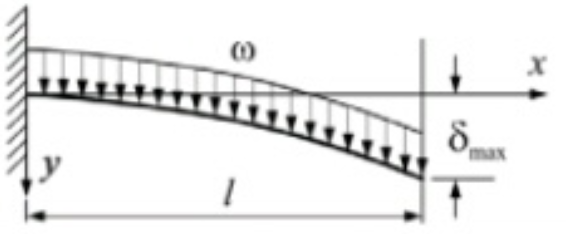
\includegraphics[width=0.5\textwidth]{beam.png}
  \caption{Ilustrasi \textit{cantilever beam}}
\end{figure}

Laporan ini secara umum mengangkat masalah \textit{vertical displacement} pada sebuah \textit{cantilever beam} yang luas momen inersia-nya konstan di sepanjang balok. \textit{Cantilever beam} sendiri merupakan struktur semacam balok dengan satu ujung tetap dan satu ujung lain bebas. Layaknya sebuah papan loncat di kolam renang. Teori Balok Euler-Bernoulli ini menetapkan suatu sistem persamaan matematika yang dapat memodelkan material ini.

Menariknya, persamaan matematika dalam permasalahan yang terlihat rumit ini ternyata dapat direduksi menjadi sebuah sistem persamaan linear, yang secara umum dapat dihitung dengan mudah melalui komputasi numerik. Lebih penting lagi, matriks koefisien yang terbentuk merupakan matriks khusus yang memiliki kompleksitas lebih cepat dibandingkan matriks lain pada umumnya. Dari latar belakang tersebut, kami akan membahas beberapa pertanyaan yang diajukan sebagai pemicu bagi proyek ini.

\section*{Isi}

Laporan ini hanya berisikan jawaban dari soal-soal yang sudah kami jawab dan analisis. Untuk referensi pertanyaan dari soal-soal tersebut telah dilampirkan pada dokumen \texttt{TK1.pdf}, pada arsip yang sama.

\subsection*{Soal 1}

Permasalahan dari latar belakang di atas dapat direduksi menjadi sistem persamaan linear sebagai berikut.

\begin{equation*}
	\begin{bmatrix}
		16 & -9 & \frac{8}{3} & -\frac{1}{4} \\
		-4 & 6 & -4 & 1 \\
		1 & -4 & 6 & -4 & 1 \\
		  & 1 & -4 & 6 & -4 & 1 \\
		  & & \ddots & \ddots & \ddots & \ddots & \ddots \\
		  & & & 1 & -4 & 6 & -4 & 1 \\
		  & & & & 1 & -4 & 6 & -4 & 1 \\
		  & & & & & \frac{16}{17} & -\frac{60}{17} & \frac{72}{17} & -\frac{28}{17} \\
		  & & & & & -\frac{12}{17} & \frac{96}{17} & -\frac{156}{17} & \frac{72}{17} \\ 
	\end{bmatrix}
	\begin{bmatrix}
	    y_1\\
	    y_2\\
	    \\
	    \vdots\\
	    \\
	    \vdots\\
	    \\
	    y_{n-1}\\
	    y_n\\
	\end{bmatrix}
	=
	\frac{h^4}{EI}
	\begin{bmatrix}
	    f(x_1)\\
	    f(x_2)\\
	    \\
	    \vdots\\
	    \\
	    \vdots\\
	    \\
	    f(x_{n-1})\\
	    f(x_n)\\
	\end{bmatrix}
\end{equation*}

Kita sudah mempelajari tentang beberapa algoritme yang bisa digunakan untuk menyelesaikan matriks-matriks \textbf{spesial} yang secara kompleksitas lebih cepat. Misalnya pada \textit{banded matrix}, kita bisa melakukan $LU$ \textit{decomposition} yang lebih \textbf{efisien}.

Caranya ialah dengan melakukan pembatasan atau \textit{pruning} contohnya seperti kode di atas. Perhatikan bahwa kompleksitas dari algoritme ini ialah sekitar $O(NPQ)$ dengan $N$ ukuran matriks, $Q$ panjang pita bawah, dan $P$ panjang pita atas. Dalam kasus ini, $P$ dan $Q$ bernilai $2$, kecuali untuk beberapa baris yang kurang sesuai (\textit{off by one})

Namun akan terjadi beberapa kesalahan, kami mengetahui hal ini karena saat mencoba memasukkan baris \texttt{[L U] = lu(A)} terjadi ketidaksesuaian. Setelah diteliti lebih lanjut, matriks ini membutuhkan \textit{pivoting} agar proses dekomposisi berhasil.

Kemudian, amati pula beberapa proses yang akan dilakukan dalam aproksimasi perhitungan ini. Pada dasarnya proses $LU$ \textit{decomposition} sama saja dengan \textit{Gaussian Elimination}. Namun pada umumnya $LU$ \textit{decomposition} digunakan karena melakukan \textit{precomputation} terhadap kedua matriks $L$ dan $U$. Sehingga saat ingin mencari solusi untuk $b$ lain, tidak perlu melakukan komputasi dengan kompleksitas $O(N^3)$ lagi. Melainkan hanya perlu melakukan \textit{forward} dan \textit{backward} substitution, dengan total kompleksitas $O(N^2)$ untuk setiap $b$ yang berbeda.

Dalam kasus ini memang agak susah dalam membuat program yang dapat melakukan \textit{row pivoting}, terutama untuk \textit{banded matrix} yang kurang sempurna pada kasus ini. Sehingga salah satu solusinya ialah dengan melakukan $LU$ \textit{decomposition} dengan \textit{partial pivoting}. Namun, akan dilakukan \textit{pruning} ketika elemen yang akan dikomputasi saat ini sudah bernilai $0$. Dalam kasus ini, masih mempertahankan kompleksitas $O(NPQ)$, dengan menambahkan suatu operasi pengecekan apakah entri bernilai $0$.

Cara lainnya ialah, langsung saja menggunakan Eliminasi Gauss. Perhatikan bahwa dengan bandwidth yang kecil, kompleksitasnya sangat mirip saat menggunakan dekomposisi $LU$ ataupun eliminasi Gauss. Bila $P$ dan $Q$ dianggap konstan, kedua operasi tersebut menghasilkan kompleksitas linear. Demi kemudahan, selain menggunakan \textit{sparse matrix}, kita bisa menggunakan matriks yang disimpan dalam \textit{compact storage}. Digunakannya \textit{compact storage} pada dasarnya akan menurunkan kompleksitas memori, dari yang awalnya menyimpan matriks banded dalam $O(N^2)$. Kini disimpan dalam $O(N+2Q+P)$. Alasan menggunakannya ialah jelas, karena kemudahan dilakukannya \textit{partial pivoting} saat melakukan Eliminasi Gauss, ataupun Dekomposisi $LU$.

\begin{figure}[h]
  \centering
    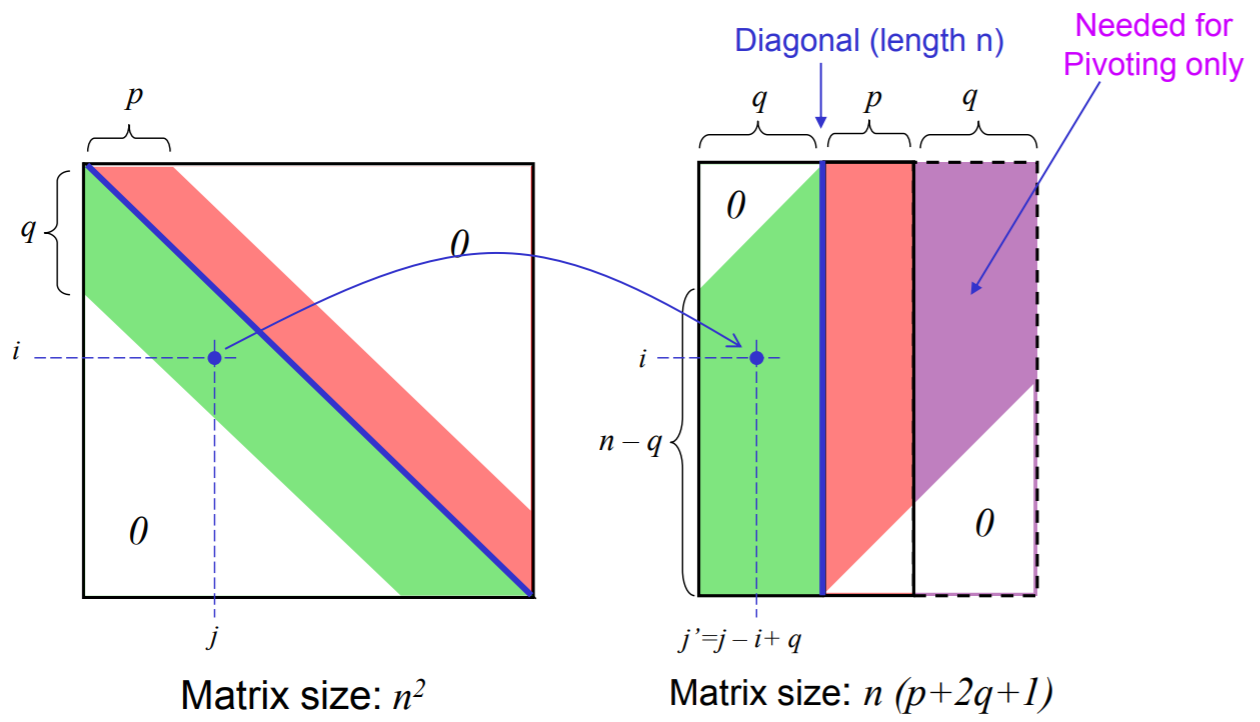
\includegraphics[width=0.5\textwidth]{Compact.png}
  \caption{Ilustrasi \textit{compact storage}}
  \textbf{Source:}  \href{https://ocw.mit.edu/courses/mechanical-engineering/2-29-numerical-fluid-mechanics-spring-2015/lecture-notes-and-references/MIT2_29S15_Lecture7.pdf}{OCW MIT 2.29 Numerical Fluid Mechanics Lecture 7 Slides}
\end{figure}

Untuk ilustrasi lebih lanjut, disertakan bersama lampiran \texttt{1\_Compact.pdf}. Perhatikan bahwa pada figur sebelah kiri ialah matriks yang akan direpresentasikan, dan sebelah kanan ialah representasi \textit{compact storage}-nya. Perhatikan bahwa saat dilakukan OBE tukar baris, penyimpanan \textit{floating point} tidak akan melebihi kolom ke-$(P+2Q+1 = 2 + 4 + 1 = 7)$. Selanjutnya, penyelesaian diimplementasikan dengan \texttt{C++} pada \texttt{1\_Beam.cpp} dan \texttt{Octave} pada \texttt{1\_Beam.m}. Didapatkan hasil yang kami buat dalam lampiran \texttt{1\_Hasil.pdf}.

\subsection*{Soal 2}
Gw kerjain soal 2 ya ok
Each exercise (except the first) starts on a new page. You can disable this behavior using the starred version of the command: \verb|\exercise*|.

Now, let's consider a mathematical example.

\subsection*{Soal 3}
Each exercise (except the first) starts on a new page. You can disable this behavior using the starred version of the command: \verb|\exercise*|.

Now, let's consider a mathematical example.

\subsection*{Soal 4}
Each exercise (except the first) starts on a new page. You can disable this behavior using the starred version of the command: \verb|\exercise*|.

Now, let's consider a mathematical example.

\nocite{*}
\bibliographystyle{apalike}
\bibliography{bibliography.bib}
\end{document}